\documentclass[utf8,12pt]{beamer}

\usepackage{graphicx}
\usepackage{amsmath}
\usepackage{bm} % bold math symbols
\usepackage{tgpagella} % Gyre pagella -- based on palatino
\usepackage[english]{babel}
\usepackage[binary-units]{siunitx}
\usepackage[absolute,overlay]{textpos}
\usepackage{verbatim}

\usetheme{default}
\usecolortheme{seagull}
\usefonttheme{serif}
\setbeamertemplate{navigation symbols}{}
\logo{\includegraphics[height=1.5cm]{img/robot.pdf}}
\setbeamertemplate{footline}
{%
\vskip-1mm
\hfill\insertsectionnavigationhorizontal{\paperwidth}{\hfill}{\hfill}
\vskip1pt
}

../text/math-defs.tex
\graphicspath{{img/}}

\title{Exploiting GPS in Monte Carlo Localization}
\author{Jakub Marek}

\begin{document}

\begin{frame}[plain]
\titlepage
\end{frame}

\section{Motivation}
\begin{frame}{Motivation}
\begin{itemize}
    \item Outdoor robots need position information
    \item Improve precision available from GPS
    \begin{itemize}
        \item Individual measurements
        \item Combination with other sensors
    \end{itemize}
    \item Improve error characterization
    \item Explore inner workings of GPS
\end{itemize}
\end{frame}

%%%% dependency img/01.jpg
%\imageframe{img/01.jpg}{black}

\begin{frame}{Why GPS}
\begin{textblock*}{3cm}[1,1](115mm,45mm)
    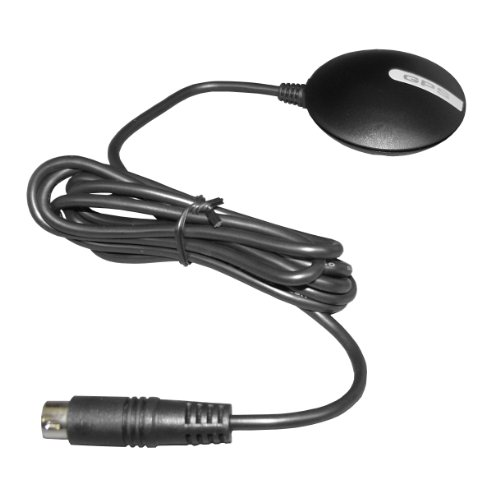
\includegraphics[height=3cm]{img/receiver.jpg}
\end{textblock*}
\begin{itemize}
    \item Worldwide absolute position
    \item No preparation required
    \item Cheap (?!)
    \item Drawbacks
    \begin{itemize}
        \item Low precision from consumer GPS receivers
        \item Low measurement frequency
    \end{itemize}
\end{itemize}
\end{frame}

{
\logo{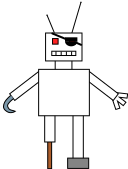
\includegraphics[height=1.5cm]{img/robot-pirate.pdf}}
\begin{frame}{Why Monte Carlo Localization}
\begin{itemize}
    \item Efficient probabilistic localization algorithm
    \item Simple to understand and implement
    \begin{itemize}
        \item Simulate a swarm of possible robots
        \item Compare the actual and simulated sensor readings
    \end{itemize}
    \item Arbitrary shapes of probability densities
    \item More computationally intensive than Kalman Filter
\end{itemize}
\end{frame}
}

\begin{frame}{Main Idea}
\begin{itemize}
    \item Utilize the GPS in MCL
    \item Improve the result using lower-level measurements
\end{itemize}
\end{frame}

\section{GPS Principles}
\begin{frame}{GPS Principles}
    \begin{itemize}
        \item Measuring time of flight of radio signals
        \begin{itemize}
            \item Ideally: position = intersection of spherical surfaces
            \item Reality: 4D conical surfaces (3D positions + time)
        \end{itemize}
        \item Pseudorange
    \end{itemize}

    \vspace{0.2cm}
    \begin{center}
    \centerline{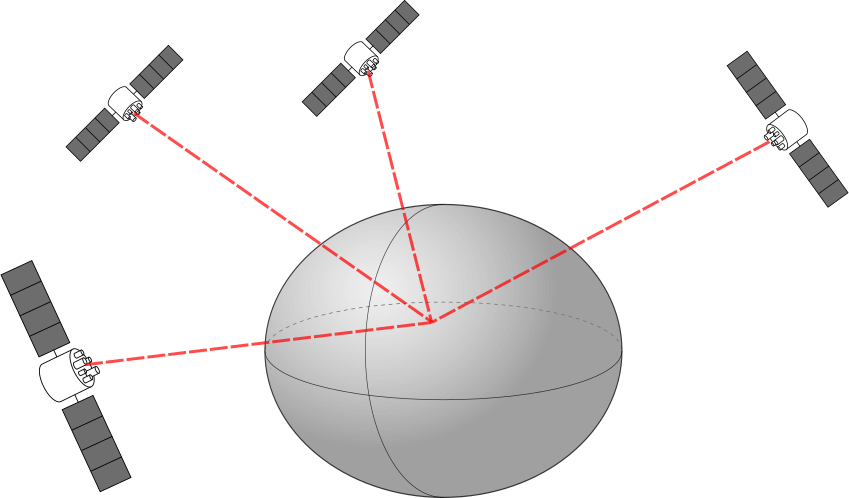
\includegraphics[height=3.8cm]{img/pseudoranges.pdf}}
    \end{center}
\end{frame}

\section{GPS and MCL -- Simple Approach}
{
\logo{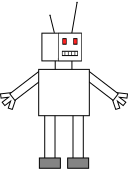
\includegraphics[height=1.5cm]{img/robot-looking-right.pdf}}
\begin{frame}[fragile]{GPS and MCL -- Simple Approach}
    \begin{itemize}
        \item Most GPS receivers provide NMEA output
        \begin{itemize}
            \item Contains WGS84 lat/lon coordinates and HDOP
        \end{itemize}
        \item Can be used as a position input almost immediately
    \item However\ldots
        \begin{itemize}
            \item Horizontal position errors only
            \item No characterization of velocity error
            \item Unknown assumptions about the platform
        \end{itemize}
    \end{itemize}

    \vspace{0.5cm}
    \begin{center}
    \small \verb=$GPGSA,A,3,04,05,,09,12,,,24,,,,,2.5,1.3,2.1*39=
    \end{center}
\end{frame}
}

\begin{frame}[plain]{Error vs. HDOP}
\begin{center}
\centerline{\includegraphics[height=8cm]{generated/wgs84-hdop-error.pdf}}
\end{center}
\end{frame}

\section{GPS and MCL -- Pseudoranges}
\begin{frame}{GPS and MCL -- Pseudoranges}
    \begin{itemize}
        \item Each pseudorange measurement as localization input
        \item Allows to use Doppler measurements
        \item Specific to a GPS chipset
        \begin{itemize}
            \item Data not in NMEA protocol
            \item SiRF III
        \end{itemize}
    \end{itemize}
\end{frame}

\begin{frame}{GPS and MCL -- Pseudoranges}
    \begin{itemize}
        \item Need to consider atmospheric delays
        \begin{itemize}
            \item Low frequency errors as a part of localization state
        \end{itemize}
        \item Approximately \SI{7}{\meter} \(1\sigma\) error for single measurement
        \begin{itemize}
            \item Similar precision to the simple NMEA data
            \item Room for improvement
        \end{itemize}
    \end{itemize}
\end{frame}

\begin{frame}[plain]{Pseudorange Errors}
\begin{center}
\centerline{\includegraphics[height=8cm]{generated/pseudorange-errors.pdf}}
\end{center}
\end{frame}

\begin{frame}{Pseudoranges vs. WGS84 Data}
    \begin{itemize}
        \item Pros
        \begin{itemize}
            \item Error characterization
            \item Velocity measurements
            \item Virtually no assumptions about the robot
            \begin{itemize}
                \item Added in prediction step of MCL
            \end{itemize}
            \item Possibility to further process measurements
            \begin{itemize}
                \item Multipath
            \end{itemize}
        \end{itemize}
        \item Cons
        \begin{itemize}
            \item Computing power
            \item More intrusive in localization algorithm
        \end{itemize}
    \end{itemize}
\end{frame}

\section{Implementation}
{
\logo{
\includegraphics[height=1.5cm]{img/robot-bottle.pdf}}
\begin{frame}{Implementation}
    \begin{itemize}
        \item Tools for analyzing GPS errors
        \begin{itemize}
            \item Recording and off-line processing
        \end{itemize}
        \item SiRF III chip
        \item Number of implementation challenges
        \begin{itemize}
            \item Documentation
            \item Clock jumps
            \item Doppler measurements
            \item Uncovered error in velocity processing
        \end{itemize}
    \end{itemize}
\end{frame}
}

\begin{frame}[plain]{Velocity Error Histogram}
\begin{center}
\centerline{\includegraphics[height=8cm]{generated/velocity-histogram.pdf}}
\end{center}
\end{frame}

\section{Conclusion}
\begin{frame}{Conclusion}
    \begin{itemize}
        \item WGS84 data
        \begin{itemize}
            \item Realistic, simple to use
        \end{itemize}
        \item Low level approach
        \begin{itemize}
            \item More complex, more flexible
        \end{itemize}
        \item Overview of GPS and SiRF
        \item Framework for further experimenting
    \end{itemize}
\end{frame}

{
\logo{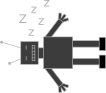
\includegraphics[width=1.5cm]{img/robot-sleep.pdf}}
\setbeamertemplate{footline}{ \hspace{1mm} }
\setbeamercolor{background canvas}{bg=black}
\begin{frame}
\end{frame}
}

{
\setbeamercolor{background canvas}{bg=black}
\begin{frame}[plain]
\end{frame}
}

\begin{frame}[plain]{Fig 2.2: Times in pseudorange measurements}
\begin{center}
\input{img/pseudorange-fixed.pdf_tex}
\end{center}
\end{frame}

%\begin{frame}[plain]
%    \centerline{\Large Thank you}
%\end{frame}
%
%\begin{frame}[plain]
%    \centerline{\Large Questions?}
%\end{frame}

\end{document}
